\documentclass[11pt, oneside]{article}   	% use "amsart" instead of "article" for AMSLaTeX format
\usepackage{geometry}                		% See geometry.pdf to learn the layout options. There are lots.
\geometry{letterpaper}                   		% ... or a4paper or a5paper or ... 
%\geometry{landscape}                		% Activate for for rotated page geometry
%\usepackage[parfill]{parskip}    		% Activate to begin paragraphs with an empty line rather than an indent
\usepackage{subcaption}
\usepackage{graphicx}				% Use pdf, png, jpg, or eps§ with pdflatex; use eps in DVI mode
								% TeX will automatically convert eps --> pdf in pdflatex	
\usepackage{gensymb}	
\usepackage{enumitem}
\usepackage{amssymb}
\usepackage{float}
\usepackage{hyperref}
\usepackage{outline}
\usepackage{textcomp}
\usepackage[utf8]{inputenc}
\hypersetup{
    colorlinks=true,
    linkcolor=blue,
    filecolor=magenta,      
    urlcolor=cyan,
}

\title{FEALink Manual}
\author{Ryan Arata}
\date{7 June 2016}							% Activate to display a given date or no date

\begin{document}
\maketitle
\tableofcontents

\section{Introduction}
FEALink is a truss solving program written by Ryan Arata and released June 2016.  The program is intended to be an educational tool used for Stanford's ENGR 14 - Intro to Solid Mechanics class.  Feel free to use, edit, and redistribute FEALink.  FEALink uses python 2.7 and finite element methods to solve for the displacement of the nodes of a truss structure.  From this information, additional metrics, such as stress, strain, and link tension, are calculated.  This displacement solution depends on the structure geometry and the material properties of each link.  As a result, don't expect FEALink's results for tension to exactly match those calculated through the method of joints or the method of sections, which does not account for material properties and assumes no deformation.

This manual goes over setting up FEALink, the usage of the FEALink interface, and a few verification problems.  To save some time and frustration using FEALink, make sure to read all the paragraphs that start with '\textbf{IMPORTANT:}'.  


\section{Getting FEALink Running}
Chances are, this is the only section of this manual you'll actually need to read (though make sure to skim for the 'IMPORTANT' parts in the rest).  The program itself is fairly intuitive to use.

FEALink is based on python 2.7 and uses the libraries numpy and matplotlib, with the GUI package Tkinter.  FEALink is also compatible (but widely untested) with python 3 - though this is not suggested.  Models created using FEALink with python 2 are not compatible with models created in python 3 and vice versa.  The example models included in the distribution are all for python 2, and will not open if you are running FEALink through python 3.  To make things easy, it is better to just use python 2.  

\textbf{IMPORTANT:} FEALink will run by opening up a terminal window (or command line on Windows).  The first time you open FEALink, it may take around a minute after the terminal window opens until the program actually opens.  This is due to your security software scanning through the program for viruses before it runs.  After the first time, it should open faster.

\subsection{Method 1 (simplest method)}
For the purpose of FEALink, the easiest method to get python 2.7 on your computer with all of the necessary libraries is to go to \url{https://www.continuum.io/downloads} and download and install the version of Anaconda for python 2.7 relevant to your operating system.  Anaconda is software package that includes a python distribution, scientific computing libraries such as numpy and matplotlib, and a whole bunch of other stuff that isn't required for running FEALink.  (Note - it's possible new versions of python will have come out since I wrote this.  Just use whatever the Anaconda python 2 version is, even if it's no longer 2.7.)  Once this is installed, you should be able to run FEALink by clicking on the relevant command file (FEALink\_Mac.command, FEALink\_Windows.bat, or FEALink\_Linux.sh).  If there are further problems, see the "Common Problems" section.

Windows users may experience additional problems and have to trouble-shoot on their own, as FEALink has had much less installation testing on Windows.

\subsection{Method 2 (Mac and Linux only)}
If you know you have python 2.7 on your computer, you \textit{can} simply install numpy and matplotlib, and then you \textit{should} be able to run FEALink.  If you feel uncomfortable with this, just install Anaconda as described in the next section.  To install these (if you don't already have them), open a terminal window and type in the following commands, pressing enter to execute each (don't include the quotations, they just indicate that everything inside is a command): 
\begin{enumerate}
	\item 'sudo easy\_install pip' (this will require a password) 
	\item 'sudo pip install numpy'
	\item 'sudo pip install matplotlib'
\end{enumerate} 

Now you should be able to run the file to open FEALink.  For further errors, see the next section.

\subsection{Common Problems} \label{Common Problems}
\begin{enumerate}
	\item{Unidentified developer}

Since I don't have any sort of software distribution license included with FEALink that your operating system will recognize, it may not allow you to run the file for security reasons.  

On mac, you can override this by going to system preference -> security \& privacy.  There should be text that says something like "mac didn't allow FEALink\_Mac.command to run because it is from an unidentified developer" and a button that says something like "run anyway."  Hit that button.

On Windows and Linux, which have less universal security systems, you may have to search online for how to override your specific security system to specifically allow FEALink to run.  Don't worry, it is safe to do this.

	\item{Not executable/Opens in text editor}

Unfortunately, some computers will be configured such that these files aren't automatically executable (this will only happen on Mac and Linux, Windows should be good).  You will know this is the case if the file opens up in some text editing program or Xcode.  Another similar common error is that you are denied permission to access or execute the file.  Luckily, these problems have the same solution.  

Open a terminal window (the terminal application).  To navigate in the terminal, there are two command you really need.  The first is 'ls', which will list all the files in the current directory.  Type 'ls' (without the quotes) into the terminal and press enter.  To change directories, use the 'cd' command.  The 'cd' command requires an argument, which is the directory you want to switch to.  For example, to move to the Desktop folder (if available as shown by 'ls'), type 'cd Desktop'.  You can go back a directory by typing 'cd ..' or back to where you started with 'cd $\sim$'.  Use these commands to navigate to the FEALink folder.  To make FEALink executable, type the following (without quotations):

'chmod a+x FEALink\_Mac.command' for mac or 'chmod a+x FEALink\_Linux.sh' for linux

If this gives you a permissions error, try 'sudo chmod a+x FEALink\_Mac.command' or 'sudo chmod a+x FEALink\_Linux.sh', then type in your password (your computer sign-on) at the prompt.  It will not show any characters when you type your password, but it is receiving them.  So just type it and press enter.  This overrides the permissions on the file to allow you to modify it.

\end{enumerate}

You should now be able to run FEALink by opening the file associated with your operating system.  If you are still experiencing issues, feel free to contact me (Ryan Arata) at \href{mailto:ryanparata@gmail.com}{ryanparata@gmail.com} with questions.

%%%%%%%%%%%%%%%%%%%%%%%%%%%%%%%%%%%%%%%%%%%%%%%%%%%%%%

\section{The FEALink Model}
FEALink is based around the concept of a Model - which is a data structure that includes all of the information necessary to solve a truss structure problem.  Models can be created in the FEALink Start Center, which is the small window that opens up when FEALink is run.  When creating or loading a model, a new window will open with an interface that allows the user to interact with and modify the model.  The primary methods by which to change the model are the "notebook" on the left, which has pages that correspond to the various attributes of the model - in the order that they generally are created in.  Each of these pages includes a listing of the information included in that model attribute (for example a list of nodes contained in the model and their locations).  In addition to the ability to interact with the model through the entry boxes and buttons in each of these pages, almost everything that can be done from the pages can also be done through the command line in the top left. To create a model, simply start at the materials tab and start moving to the right from there.  The plot on the right will update as new nodes, links, constraints, and forces are created.  Labels on the plot can be toggled with the checkboxes in the top right of the interface.  Whenever there is an error with any action, a red label will pop up within the relevant page window, displaying the error for 2.5 seconds.

\subsection{Saving/Loading Models}
Models can be saved at any point during their creation.  The 'Save Model' button is in the top right of the model window.  Alternatively, the 'save' command can be performed in the command line (not case sensitive) or through the 'File' menu.  Either of these methods will open up a save dialog where the model can be named and placed in the desired directory.  

\textbf{IMPORTANT:} Models cannot be opened by simply clicking on the file through Finder/Windows Explorer/some other directory manager.  Models must be opened from the FEALink start center 'Load Model' or through the 'File' menu when focus is on the start center.  The files that FEALink saves contain only information about the model, not about the FEALink program that opens the model and allows interaction with it.

\subsection{Notes}
The 'Notes' tab contains entries for model units and a general notes text box.  Start by defining the units that the model will be defined in in this tab.  Default is SI units.

\textbf{IMPORTANT:} The units input into the notes tab don't actually mean anything to the model.  It is up to the user to ensure that they input all values in a consistent unit scheme.  The boxes in the notes tab simply help keep track of what units the model is in for reference.  The results will come out in the same units as the input - regardless of whether that matches the units shown in the notes or not.

\subsection{Materials}
FEALink allows multiple materials to exist in the same model.  These materials are later associated to each link in the truss structure.  Each Material is labeled by a unique integer, and contains information about the cross-sectional area and elastic modulus of the material.  Filling in the three entry boxes under the 'Make New Material' button and pressing the button or hitting enter while the focus is in one of those three entry boxes will create a new material (or show an error message).  Materials can be deleted by number with the entry box under the 'Delete Material' button.  It is optional to include the density of a material.  If it is included, it allows FEALink to calculate mass properties when it solves the structure.

The list of existing materials is updated whenever a material is added or deleted, and can be seen in the listing on the Material page.  This table is scrollable if the list exceeds the height of the widget.  In some cases, you may have to click on the list widget to give it focus in order for it to scroll.  

\textbf{IMPORTANT:} In any of the entry boxes, numbers can be entered in scientific notation through the format as shown by this example: '1e-6' (don't include the quotes).  Python will interpret this as 0.000001.  This comes in handy when Young's Modulus is something like 2e11.

If you attempt to create a material with the same number as a material that already exists, the existing material will be replaced, and a warning will be shown.

The command line commands for creating and deleting nodes are:

\begin{equation}
m, MaterialNumber, Area, YoungsModulus
\end{equation}

\begin{equation}
dm,MaterialNumber1,MaterialNumber2,MaterialNumber3,etc...
\end{equation}

The 'dm' command can also be used with the Matlab list format of $ dm, FirstNum:Increment:LastNum $ or $ dm, FirstNum:LastNum $ to have an increment of 1 (delete nodes between and including those two numbers).  Material numbers do not have to be explicitly defined, but there must be a space between commas for it.  If the space between the first and second comma in the material creation command is blank, it will be auto-numbered.  For example, $m, , 1e-3,4e9$ creates an auto-numbered material.

\subsection{Nodes}
Nodes are the basis of the truss structure.  In statics, they are often referred to as joints - they can transmit forces but no moments.  Anywhere that Links will start or end, there needs to be a node.  Creating and deleting nodes is much the same as materials.  The MultiNode tool at the bottom of the node page allows the user to create multiple nodes in a line at once.  The nodes created are evenly spaced between (StartX,StartY) and (EndX,EndY), or (StartX,StartY,StartZ) and (EndX,EndY,EndZ) in 3d.  The first node number is indicated by the 'First Node \#' box, and are labelled with numbers spaced out as defined in the 'Node \# Spacing' box.  If all of the nodes are at the same location in one dimension, the 'End' condition in that dimension need not be specified - it will be defaulted to the same value as the 'Start' condition.

Like materials, redefining a node will replace the node and move it to the new position, maintaining connection to all attached links.

Command line for creating a node, deleting nodes, and using MultiNode:

\begin{equation}
n, NodeNumber, X, Y, Z
\end{equation}

\begin{equation}
dn, NodeNumber1, NodeNumber2, NodeNumber3, etc...
\end{equation}

\begin{equation}
mn, FirstNodeNum, NumNodes, NodeNumSpacing, StartX, EndX, StartY, EndY, StartZ, EndZ
\end{equation}

Like materials, multi-node deletion can be achieved with the colon-based list format as well.  In 2d, all of the 'Z' portions can be omitted.  Again, like in materials, the node number can be unspecified and well be auto-assigned.  

\subsection{Links}
Links are what physically make up the model.  The link is defined between two nodes, and must have an associated material.  If not specified, the material will default to material \# 0.  The MultiLink tool allows links to be created between all nodes which have node numbers spaced apart by a certain value.  This can save some time in model creation, but is also to be used with caution, because it may create links you don't notice.  For example if nodes 1, 2, and 3 are all in a line and node 1 is connected to 2 and 2 is connected to 3, and your MultiLink creates a link between 1 and 3, it may go unnoticed but significantly effect the stiffness of the model in that area.  

Command line for creating a link, deleting links, and using MultiLink:

\begin{equation}
l, LinkNumber, Node1, Node2, MaterialNumber
\end{equation}

\begin{equation}
dl, LinkNum1, LinkNum2, LinkNum3, etc...
\end{equation}

\begin{equation}
ml, 1stLinkNum, LowNodeNum, HighNodeNum,  MaterialNum, NodeSpacing, LinkSpacing
\end{equation}

For creating a link, the material can be omitted in order to use the default material number 0.  For MultiLink, any or all of the last three entries can be left out, with defaults of MaterialNum = 0, NodeSpacing = 1, LinkSpace = 1.

\subsection{Constraints and Forces}
FEALink supports both zero and non-zero displacements in the x-, y-, and z-directions.  It does not allow for a displacement constraint on a line or plane that is not aligned with one of the axes.  

\textbf{IMPORTANT:} To define a constraint, put values only in the boxes where there is a constraint and leave the rest blank.  For example, a roller constraint that can move in the x-direction and not the y-direction would have a 0 in the 'y displacement' box and nothing in the 'x displacement' box.  

The same goes for the command line command.  Zero displacements will be shown graphically in cyan, while nonzero constraints are shown in magenta.  

Constraint commands:

\begin{equation}
c, NodeNum, Xdisplacement, Ydisplacement, Zdisplacement
\end{equation}

\begin{equation}
dc, NodeNum1, NodeNum2, NodeNum3, etc...
\end{equation}

Forces are placed on nodes, just as constraints are.  They are defined via their x-, y-, and z- components, which are defaulted to 0 if blank.  Forces are shown graphically with red arrows - the length of which indicates the relative magnitude compared to other forces in the model.

Force commands:

\begin{equation}
f, NodeNum, Xcomponent, Ycomponent, Zcomponent
\end{equation}

\begin{equation}
df, NodeNum1, NodeNum2, NodeNum3, etc...
\end{equation}

\subsection{Solution and Output}
FEALink uses Finite Element Analysis to solve for the resulting nodal displacements of the model - then calculates information about tension, stress, and strain from the displacement.  As a result, the numbers that come out will be slightly different than those that are solved for by the method of section or the method of joints - though FEALink will converge to those solutions with very thick or stiff materials.  In addition, the methods used to enforce boundary conditions allow for tiny errors in the exact location of constrained nodes in order to solve the system of equations.  Nodal displacements that are several orders of magnitude less than the others generally mean those displacements are zero.  The command for solve is:

\begin{equation}
s
\end{equation}

Commanding this or hitting the solve button will bring attention to the solution page and either update the solution tables or give an error.  When solving a FEALink problem, the system must statically stable, and must have at least one constraint in every direction in which a force acts.  There can be some frustration involved in converting a model that works in 2 dimension to 3 dimension.  A lot more constraints or links are required for the problem to fit the stability equation ($d*n \leq l+c$, where n = number of nodes, l = number of links, and c = number of constraints) in 3d than in 2d.  In addition, not all models that satisfy this equation are actually stable and solvable.  Model systems in 2d when possible.  This is not to say 3d models don't work - just that 3d models should be used for problems that are inherently 3d.

\textbf{IMPORTANT:} FEALink does not update the solution of the model until the 'Solve' button is pressed or the solve command is run.  Changes in the model will not be reflected in the solution - either the listings or the plot - until it is updated with a new solve.

The solution can be plotted in a couple ways using the check boxes inside the solution page.  Stresses can be shown on the solution plots (either exaggerated or exact) by a color-coding.  Tension ranges from black (0 tension) to bright red (maximum tension link), while compression ranges from black (0 compression) to bright green (maximum compression link).  A key for what these values are is shown at the top of the plot when the 'Show Stress' box is checked.

\subsection{Plot}
The plotting interface is based on the python library matplotlib.  In 2d, the toolbar on the bottom can help navigate the view of the model.  Hold your mouse over a button to see what it does.  You can save images of your plot with this toolbar, as well.

Unfortunately, not all of the elements of the toolbar work for 3d models (this is a deficiency of the library), but there are a few helpful ways to navigate.  Holding the left mouse button and dragging will change the model orientation, and holding the right mouse button and dragging up or down will zoom in and out.  

The display of numbering, forces, and constraints can be toggled with the checkboxes above the plot.  In addition, different displays of results are available one the model has been solved.  These can be found under the 'Solution' page.

%%%%%%%%%%%%%%%%%%%%%%%%%%%%%%%%%%%%%%%%%%%%%%%%%%%%%%

\section{FEALink Command Line}
The entry box in the top left of the model window is called the command line.  Most actions that can be performed on the model have a command sequence that can replicate that command, speeding up the process of modeling by circumventing GUI navigation.  The command line saves previous commands entered into it, and they can be accessed by pressing the up arrow key when the cursor is in the entry box.

The following list shows all of the commands available through the command line and their syntax.  Anything in brackets is an optional argument.  Optional arguments in the middle of a command must still have a comma space where they would otherwise exist (except for z-values, which do not need to be present at all in 2-d models - these are shown in parentheses), while optional arguments at the end can be entirely omitted.  The first element in any command is called the command type, and there are generally multiple letter/word sequences that work for the same command.  In addition, commands may have multiple possible syntaxes.

\begin{itemize}
 \item{Create Material: 'm' / 'material'} 
 	\begin{itemize}
 		\item m, [Num=next], Area, Modulus
	\end{itemize}
 \item{Delete Material: 'dm' / 'deletematerial'}
 	\begin{itemize}
 		\item dm, Num1, [Num2,...]
		\item dm, FirstNum:Increment:LastNum
		\item dm, FirstNum:LastNum
	\end{itemize}
 \item{Create Node: 'n' / 'node' / 'createnode' / 'newnode'}
 	\begin{itemize}
 		\item n, [Num=next], x, y(, z)
	\end{itemize}
\item{Delete Node: 'dn' / 'deletenode'}
 	\begin{itemize}
 		\item dn, Num1, [Num2,...]
		\item dn, FirstNum:Increment:LastNum
		\item dn, FirstNum:LastNum
	\end{itemize}
 \item{Create Link: 'l' / 'link' / 'createlink' / 'newlink'}
 	\begin{itemize}
 		\item l, [Num=next], NodeNum1, NodeNum2
	\end{itemize}
\item{Delete Link: 'dl' / 'deletelink'}
 	\begin{itemize}
 		\item dl, Num1, [Num2,...]
		\item dl, FirstNum:Increment:LastNum
		\item dl, FirstNum:LastNum
	\end{itemize}
\item{Add Constraint: 'c' / 'd' / 'constrain' / 'constraint' / 'displacement/}
	\begin{itemize}
		\item c, NodeNum, [x=None], [y = None](, [z = None])
	\end{itemize}
\item{Delete Constraint: 'dc' / 'dd' / 'deleteconstraint' / 'deleteconstrain' / 'deletedisplacement'}
 	\begin{itemize}
 		\item dl, Num1, [Num2,...]
		\item dl, FirstNum:Increment:LastNum
		\item dl, FirstNum:LastNum
	\end{itemize}
\item{Add Force: 'f' / 'force' / 'addforce'}
	\begin{itemize}
		\item c, NodeNum, [x=0], [y = 0](, [z = 0])
	\end{itemize}
\item{Delete Force: 'df' / 'deleteforce'}
 	\begin{itemize}
 		\item dl, Num1, [Num2,...]
		\item dl, FirstNum:Increment:LastNum
		\item dl, FirstNum:LastNum
	\end{itemize}
\item{MultiNode: 'mn' / 'multinode' / 'linnode' / 'linearnode'}
	\begin{itemize}
		\item mn, [FirstNodeNum = next], NumberOfNodes, [NodeNumberSpacing = 1], startX, [endX = startX], startY, [endY = startY](, startZ, [endZ = startZ])
	\end{itemize}
\item{MultiLink: 'ml' / 'multilink'}
	\begin{itemize}
		\item ml, [FirstLinkNum = next], [NodeNumLowerBound = 0], [NodeNumUpperBound = lastLink], [MaterialNum = 0], [NodeNumSpacing = 1], [LinkNumSpacing = 1]
	\end{itemize}
\item{Solve: 's' / 'solve'}
	\begin{itemize}
		\item s
	\end{itemize}
\item{Toggle Node Numbers: 'nn' / 'nodenumbers'}
	\begin{itemize}
		\item nn
	\end{itemize}
\item{Toggle Link Numbers: 'ln' / 'linknumbers'}
	\begin{itemize}
		\item ln
	\end{itemize}
\item{Toggle Show Force: 'sf' / 'showforce' / 'showforces'}
	\begin{itemize}
		\item sf
	\end{itemize}
\item{Toggle Show Constraints: 'sc' / 'showconstrain' / 'showconstraint' / 'showconstraints'}
	\begin{itemize}
		\item sc
	\end{itemize}
\item{Save: 'save'}
	\begin{itemize}
		\item save
	\end{itemize}
\item{SaveAs: 'saveas'}
	\begin{itemize}
		\item saveas
	\end{itemize}
\item{Update Plot (replot): 'up' / 'rp' / 'plot' / 'update' / 'updateplot' / 'replot'}
	\begin{itemize}
		\item up
	\end{itemize}
\item{Toggle Exaggerated Deformation Plot: 'pe' / 'ex' / 'plotexaggerated' / 'ed' / 'exaggerateddeformation' / 'exag' / 'ped' / 'plotexaggerateddeformation'}
	\begin{itemize}
		\item pe
	\end{itemize}
\item{Toggle Results Plot: 'pr' / 'plotresult' / 'plotresults' / 'sr' / 'showresult' / 'showresults' / 'per' / 'plotexact' / 'plotexactresults'}
	\begin{itemize}
		\item pr
	\end{itemize}
\item{Toggle Model Plot (if other plot shown): 'p' / 'pm' / 'plotmodel' / 'show' / 'showmodel' / 'sm' / 'plotpreloadedmodel' / 'ppm' / 'pplm'}
	\begin{itemize}
		\item p
	\end{itemize}
\item{Toggle Show Stress: 'ss' / 'showstress' / 'ps' / 'plotsress'}
	\begin{itemize}
		\item ss
	\end{itemize}
\item{Quit: 'q' / 'quit'}
	\begin{itemize}
		\item q
	\end{itemize}
\end{itemize}


%%%%%%%%%%%%%%%%%%%%%%%%%%%%%%%%%%%%%%%%%%%%%%%%%%%%%%

\section{Verification}
In order to verify the results of FEALink, I tested it with multiple arbitrary cases against results from a number of sources.  These sources include hand calculations via the method of nodes, results from the Johns Hopkins online truss solver tool (which also uses the method of nodes), and ANSYS (a commercial finite element package). 

\subsection{2d Verification 1}
The first verification problem is a simply supported triangular truss with a horizontal load on the point of the triangle, as shown in figure \ref{fig:V1FEALink}.  Note that the shown deflection is an exaggerated version of the actual deflection.  Red links are in tension and green are in compression.  A similar plot produced by Ansys is shown in figure \ref{fig:V1Ansys}, also with an exaggerated deformation.  For FEALink and Ansys, material and section properties are: $ A = 10^{-4} m^2 $, $ E = 2*10^{11} Pa $, $ \lambda = 0 $.

\begin{figure}[h]
\centering
  \begin{subfigure}[b]{0.45\textwidth}
    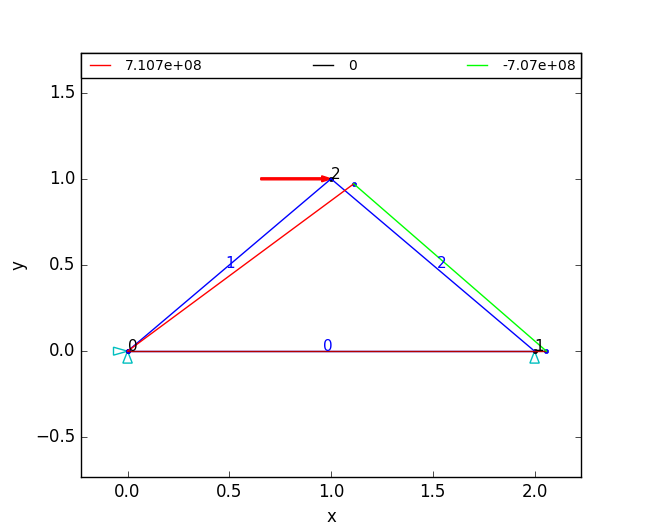
\includegraphics[width=\textwidth]{Verification/FEALink/Verification1.png}
    \caption{FEALink}
    \label{fig:V1FEALink}
  \end{subfigure}
  %
  \begin{subfigure}[b]{0.45\textwidth}
    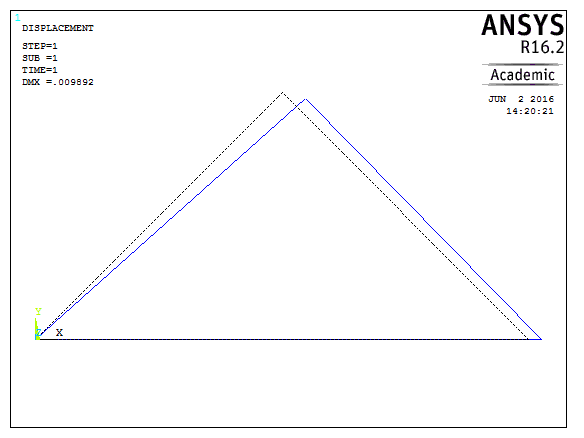
\includegraphics[width=\textwidth]{Verification/Ansys/Verification1.png}
    \caption{Ansys}
    \label{fig:V1Ansys}
  \end{subfigure}
\caption{Verification 1}
\label{fig:Verification1}%
\end{figure}

I checked this very simple example using both Ansys and solving by hand using the method of joints shown below:

\begin{equation}
F_x(2) = 0 = 100,000 - T_1\cos(45\degree) + T_2\cos(45\degree)
\end{equation}
\begin{equation}
F_y(2) = 0 = -T_1\sin(45\degree) - T_2\sin(45\degree)
\end{equation}
\begin{equation}
-> T_1 = 70,710.7 N
\end{equation}
\begin{equation}
-> T_2 = -70,710.7 N 
\end{equation}
\begin{equation}
F_x(1) = 0 = -T_2\cos(45\degree) - T_0
\end{equation}
\begin{equation}
F_y(1) = 0 = R_{1y} + T_2\sin(45\degree)
\end{equation}
\begin{equation}
-> T_0 = 50,000 N
\end{equation}
\begin{equation}
-> R_{1y} = 50,000 N
\end{equation}
\begin{equation}
F_x(0) = 0 = R_{0x} + T_0 + T_1\cos(45\degree)
\end{equation}
\begin{equation}
F_y(0) = 0 = R_{0y} + T_1\sin{45\degree}
\end{equation}
\begin{equation}
-> R_{0x} = -100,000 N
\end{equation}
\begin{equation}
 -> R_{0y} = -50,000 N
\end{equation}

The results from this method of joints, Ansys, and FEALink are tabulated in table \ref{table:V1}.  Note that the method of joints assumes no deformation in the model, while FEALink calculates tension by first calculating displacement, then getting strain, stress, and tension in each link as a result of the deformation.  This means that, as the stiffness of the links approaches infinity (stiffness defined by $\frac{AE}{L}$), the tensions should (and do) approach those calculated by the method of nodes.  It is interesting to note that Ansys calculates displacement and tension separately for link elements, resulting in displacements that exactly match FEALink and tensions that closely match the analytical result.  

\begin{table}
\centering
\caption{Verification 1 Data}
\label{table:V1}
\begin{tabular}{l|l|l|l}
          & Method of Joints & Ansys        & FEALink    \\ \hline
$T_0$      & 50,000 N         & 50,000 N     & 50,000 N   \\
$T_1$      & 70,710.7 N       & 71,073.8 N   & 70,711 N   \\
$T_2$      & -70,710.7 N      & - 70,700.0 N & -70,711 N  \\
$R_{0x}$ & -100,000 N       & -100,000 N   & -100,000 N \\
$R_{0y}$ & -50,000 N        & -50, 000 N   & -50,000 N  \\
$R_{1y}$ & 50,000 N         & 50,000 N     & 50,000 N   \\
$U_{0x}$ & N/A              & 0 m           & 0 m         \\
$U_{0y}$ & N/A              & 0 m           & 0 m         \\
$U_{1x}$ & N/A              & .005 m        & .005 m      \\
$U_{1y}$ & N/A              & 0 m           & 0 m         \\
$U_{2x}$ & N/A              & 9.57E-3 m     & 9.57E-3 m   \\
$U_{2y}$ & N/A              & -2.5E-3 m     & -2.5E-3 m  
\end{tabular}
\end{table}

FEALink's inexact adherence to analytical results in terms of tension is not error - just a difference in method. It may, in fact, be closer to the true solution, because it takes into account material properties and the deformation of the structure (as long as the deformations are small).  The calculation of tension from displacement is very simple, and the displacement results exactly match those output by Ansys.


\subsection{2d Verification 2}
The second verification problem is from the bridge that I (Ryan Arata) personally created for ENGR 14.  The design is called a k-truss.  This bridge design was built out of balsa wood, which has an approximate modulus of elasticity of $ E = 4*10^9 Pa = 4*10^7 \frac{kg}{s^2 cm} $ and the cross-sectional area was $ A = (3.175 mm)^2 = .1008 cm^2 $.  The bridge is 12cm long, making it a perfect opportunity to test FEALink using alternative units (cm instead of m in all aspects of the design).  The forces of 25N each that are placed on the three nodes in the center of the bottom of the bridge are then $ 2500 \frac{kg cm}{s^2} $. 

\begin{figure}
\centering
  \begin{subfigure}[b]{0.45\textwidth}
    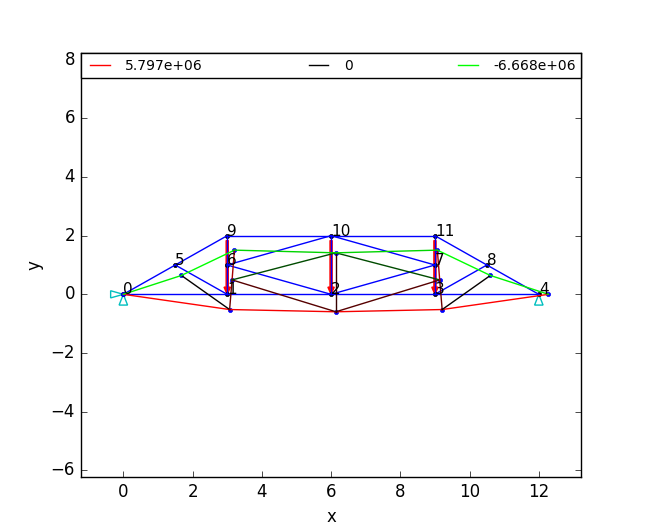
\includegraphics[width=\textwidth]{Verification/FEALink/Verification2.png}
    \caption{FEALink}
    \label{fig:V2FEALink}
  \end{subfigure}
  %
  \begin{subfigure}[b]{0.45\textwidth}
    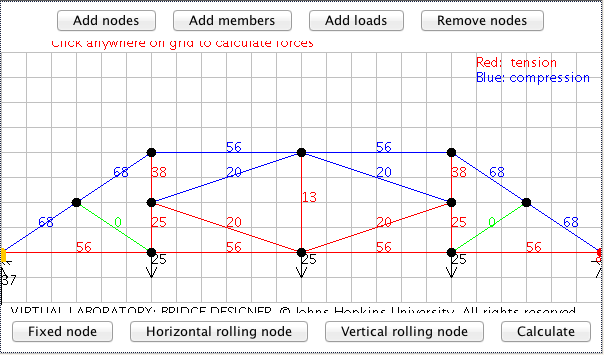
\includegraphics[width=\textwidth]{Verification/JH/Verification2.png}
    \caption{Johns Hopkins Solver}
    \label{fig:V2JH}
  \end{subfigure}
  %
  \begin{subfigure}[b]{.45\textwidth}
   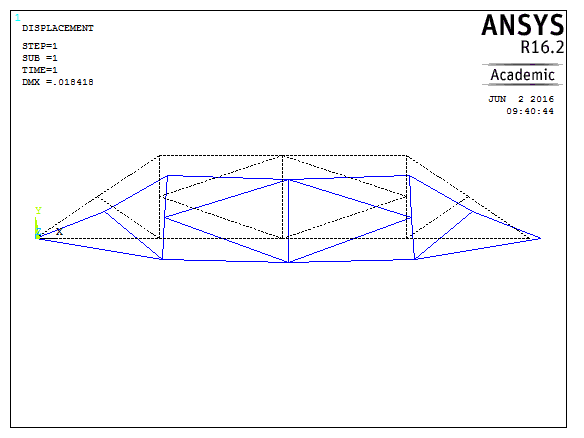
\includegraphics[width=\textwidth]{Verification/Ansys/Verification2.png}
   \caption{Ansys}
   \label{fig:V2Ansys}
  \end{subfigure}
\caption{Verification 2}
\label{fig:Verification2}%
\end{figure}

In addition to FEALink, I tested this verification model on Ansys and the Johns Hopkins online truss solver that ENGR 14 students have traditionally used (and that I used when I took the class).  Results are shown in table \ref{table:V2}.  Again, FEALink solves for link tension in a different (and possibly more accurate) way than does the method of joints, resulting in some disparities.  The displacements, however, exactly match the Ansys results (and thus are not worth tabulating here), indicating that the solution is indeed correct.  Note that FEALink and Ansys output in $\frac{kg cm}{s^2}$, but this table is converted to Newtons.

\begin{table}[]
\centering
\caption{Verification 2 Data}
\label{table:V2}
\begin{tabular}{l|l|l|l}
Link Number/Reaction & Johns Hopkins & FEALink    & Ansys \\ \hline
0           & 56 N             & 58.44 N  & 56.25 N  \\
1           & 56 N             & 56.30 N  & 56.25 N  \\
2           & 56 N             & 56.30 N  & 56.25 N  \\
3           & 56 N             & 58.44 N  & 56.25 N  \\
4           & -68 N            & -64.08 N & -67.60 N \\
5           & 0 N              & 0.86 N   & 0 N      \\
6           & 25 N             & 25.37 N  & 25 N     \\
7           & 20 N             & 19.81 N  & 20 N     \\
8           & 20 N             & 19.81 N  & 20 N     \\
9           & 25 N             & 25.37 N  & 025 N    \\
10          & 0 N              & 0.86 N   & 0 N      \\
11          & -68 N            & -64.08 N & -67.60 N \\
12          & -68 N            & -67.22 N & -67.60 N \\
13          & 38 N             & 37.84 N  & 37.5 N   \\
14          & -20 N            & -19.73 N & -19.76 N \\
15          & 13 N             & 12.5 N   & 12.5 N   \\
16          & -20 N            & -19.73 N & -19.76 N \\
17          & 38 N             & 37.83 N  & 37.5 N   \\
18          & -68 N            & -67.22 N & -67.60 N \\
19          & -56 N            & -56.18 N & -56.25 N \\
20          & -56 N            & -56.18 N & -56.25 N \\
$R_{0x}$& 0                & 0        & 0        \\
$R_{0y}$& 37.5 N           & 37.5 N   & 37.5 N   \\
$R_{4y}$& 37.5 N           & 37.5 N   & 37.5 N  
\end{tabular}
\end{table}


\subsection{2d Verification 3}
Verification 3 is a simple test of solving a statically indeterminate problem - something the method of joints cannot achieve, and therefore the Johns Hopkins software cannot do.  Instead, I tested the displacement results against Ansys.  They are a perfect match, as in all other cases.

\begin{figure}[h]
\centering
  \begin{subfigure}[b]{0.45\textwidth}
    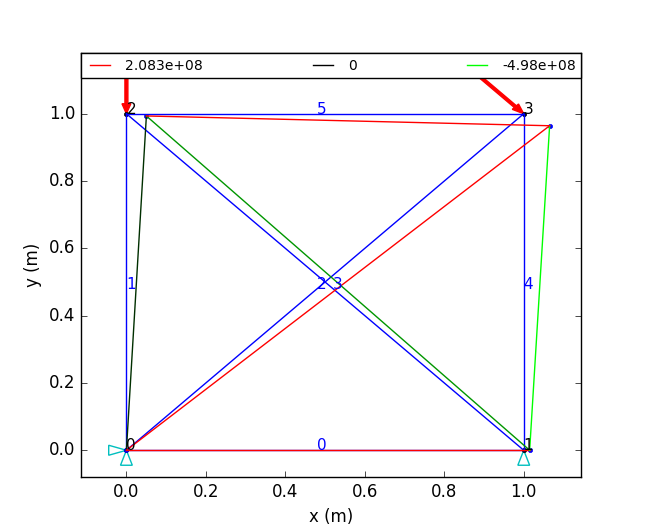
\includegraphics[width=\textwidth]{Verification/FEALink/Verification3.png}
    \caption{FEALink}
    \label{fig:V3FEALink}
  \end{subfigure}
  %
  \begin{subfigure}[b]{0.45\textwidth}
    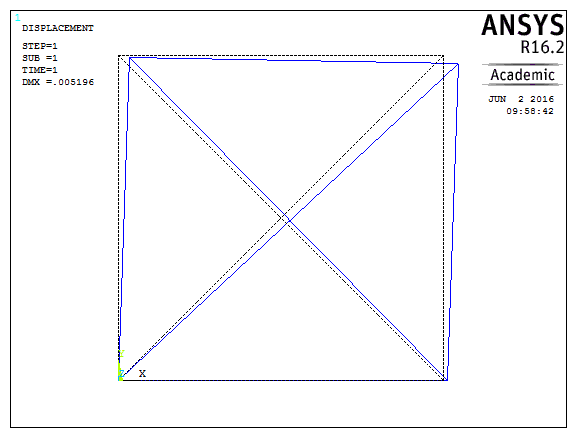
\includegraphics[width=\textwidth]{Verification/Ansys/Verification3.png}
    \caption{Ansys}
    \label{fig:V3Ansys}
  \end{subfigure}
\caption{Verification 3}
\label{fig:Verification3}%
\end{figure}

\begin{table}[h]
\centering
 \caption{Verification 3 Displacement}
 \label{table:V3}
 \begin{tabular}{l|l|l|l|l}
 Node & FEALink x & FEALink y  & Ansys x   & Ansys y    \\ \hline
 0    & 0 m       & 0 m        & 0 m       & 0 m        \\
 1    & .001039 m & 0 m        & .001039 m & 0 m        \\
 2    & .003518 m & -.000461 m & .003518 m & -.000461 m \\
 3    & .004557 m & -.002496 m & .004557 m & -.002496 m   
 \end{tabular}
\end{table}

\subsection{Invalid Model Verification}
To help ensure that FEALink doesn't have any unexpected behavior, I tested a few structures that are ill-defined.

\textbf{Invalid model A:} This model, shown in figure \ref{fig:InvalidA} is a simple unstable structure.  As expected (and designed), FEALink fails to solve it, showing the error message: "Error: Unstable structure - check constraints."

\begin{figure}[!h]
\centering
 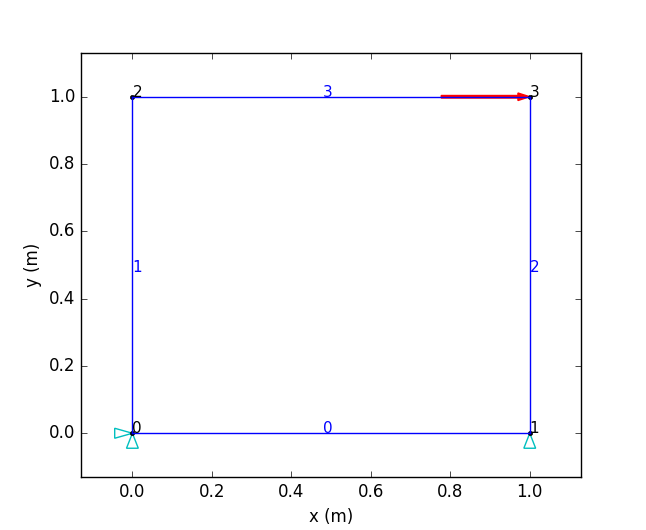
\includegraphics[width=.5\textwidth]{Verification/FEALink/InvalidA.png}
 \caption{Invalid Model A}
 \label{fig:InvalidA}
\end{figure}

\textbf{Invalid model B:} This model, shown in figure \ref{fig:InvalidB}, satisfies the equation for truss structure stability, but is still dynamically unstable, as it is not constrained in the direction in which a force is applied.  FEALink shows the error: "Error: problem is insufficiently constrained."

\begin{figure}[!h]
\centering
 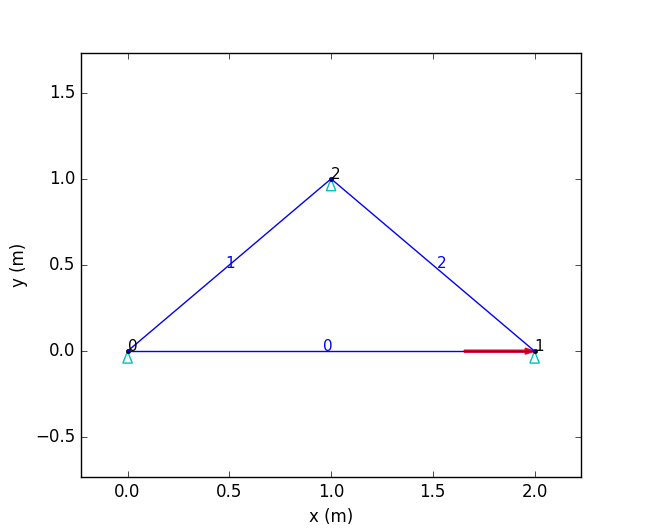
\includegraphics[width=.5\textwidth]{Verification/FEALink/InvalidB.png}
 \caption{Invalid Model B}
 \label{fig:InvalidB}
\end{figure}

\textbf{Invalid Model C:} This model, shown in figure \ref{fig:InvalidC} shows the response of FEALink to a similar structure to B, but with the force in a constrained direction.  FEALink again fails with the error "Solve Failed," because there is no stiffness in the x-direction to define the displacement.  This, while not necessarily the desired behavior, is expected, and can be rectified by simply adding an x-constraint to get the desired result.  However, placing a force on a constrained node in the direction of the node is foolish in the first place, resulting in non-zero displacements where there really should be no displacement at all.

\begin{figure}[!h]
\centering
 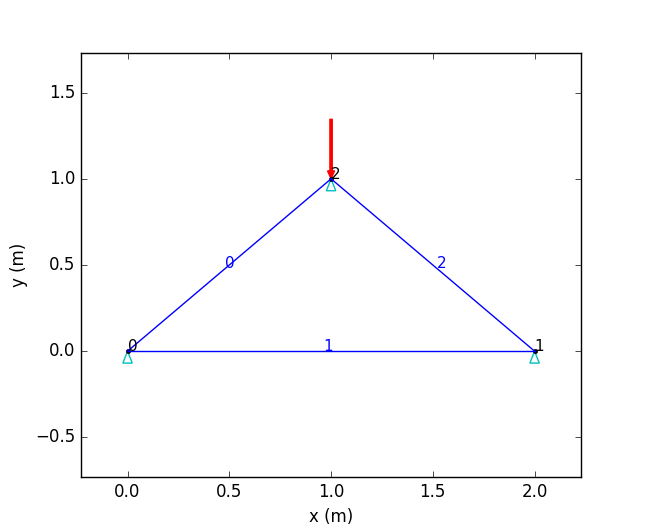
\includegraphics[width=.5\textwidth]{Verification/FEALink/InvalidC.png}
 \caption{Invalid Model C}
 \label{fig:InvalidC}
\end{figure}


\subsection{3d Verification 1}
This verification compares a 3D model against the Ansys displacement results.  There are two additional new features to this model: the load is by means of a displacement constraint (move the top node up by 1cm), and the links have different properties.  See table \ref{table:3dV1Material} for link material properties.  As in all other cases, they are the same to a very high level of accuracy.  See figures \ref{fig:3dV1FEALink} and \ref{fig:3dV1Ansys} and table \ref{table:3dV1}.  

It is worthy of note that, like Ansys, FEALink actually calculates non-zero displacements for constrained node-directions due to what is called the Penalty Method in Finite Element Analysis.  However, these displacements are several orders of magnitude lower than other displacements, (and really should be zero), so FEALink outputs them as the constrained value rather than the calculated value.

\begin{table}[h]
\centering
 \caption{3d Verification 1 Materials}
 \label{table:3dV1Material}
 \begin{tabular}{l|l|l}
 Link & Area (m\textasciicircum 2) & Young's Modulus (Pa) \\
 0-3 & 1E-3                       & 1E9                  \\
 5    &  1E-4                       & 2E11                 \\
 6    & 1E-3                       & 2E11                 \\
 7    & 1E-4                       & 5E10                 \\
 8    & 1E-3                       & 5E10       
 \end{tabular}
\end{table}

\begin{figure}[h]
\centering
  \begin{subfigure}[b]{0.45\textwidth}
    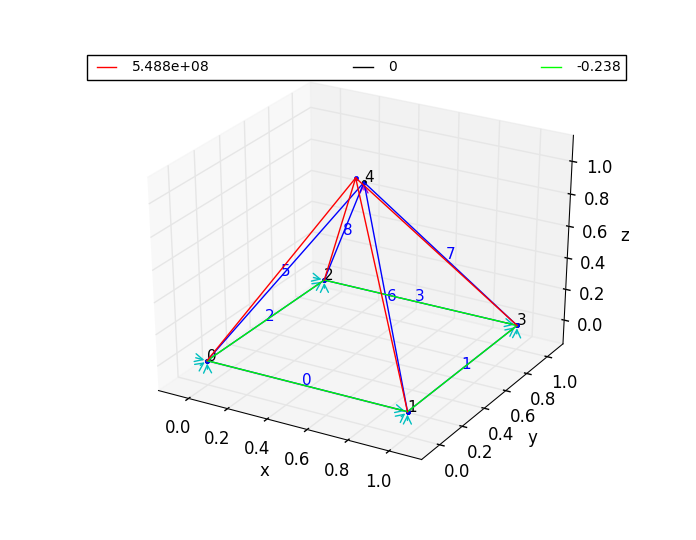
\includegraphics[width=\textwidth]{Verification/FEALink/3dVerification1.png}
    \caption{FEALink}
    \label{fig:3dV1FEALink}
  \end{subfigure}
  %
  \begin{subfigure}[b]{0.45\textwidth}
    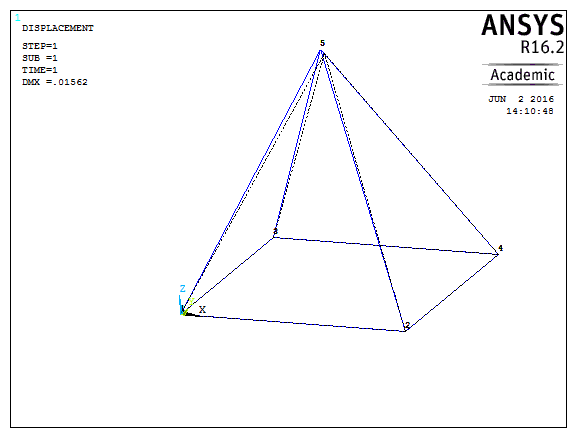
\includegraphics[width=\textwidth]{Verification/Ansys/3dVerification1.png}
    \caption{Ansys}
    \label{fig:3dV1Ansys}
  \end{subfigure}
\caption{3d Verification 1}
\label{fig:3dVerification1}%
\end{figure}

\begin{table}[h]
\centering
 \caption{3d Verification 1 displacement}
 \label{table:3dV1}
 \begin{tabular}{l|l|l|l|l|l|l}
 Node & FEALink x           & FEALink y & FEALink z & Ansys x    & Ansys y & Ansys z \\ \hline
 0-3  & 0 m                  & 0m         & 0m         & 0m          & 0m       & 0m       \\
 4     & 0m                   & -.012m     & -.01m      & -1.185E-10 $\approx$ 0m & .012m    & -.01m  
 \end{tabular}
\end{table}


\subsection{3d Verification 2}
This model tests static indeterminacy in 3d, comparing the FEALink results to Ansys results.  The verification is a success, as the results are the same.  This model uses a material with $E = 4*10^9 Pa$ and $A = 1*10^{-6} m^2$.  There is a force of 100 N in the positive y direction on node 4 and a force of 100 N in the negative Y direction on node 5.  Refer to figure \ref{fig:3dV2FEALink1}.

\begin{figure}[H]
\centering
  \begin{subfigure}[b]{0.45\textwidth}
    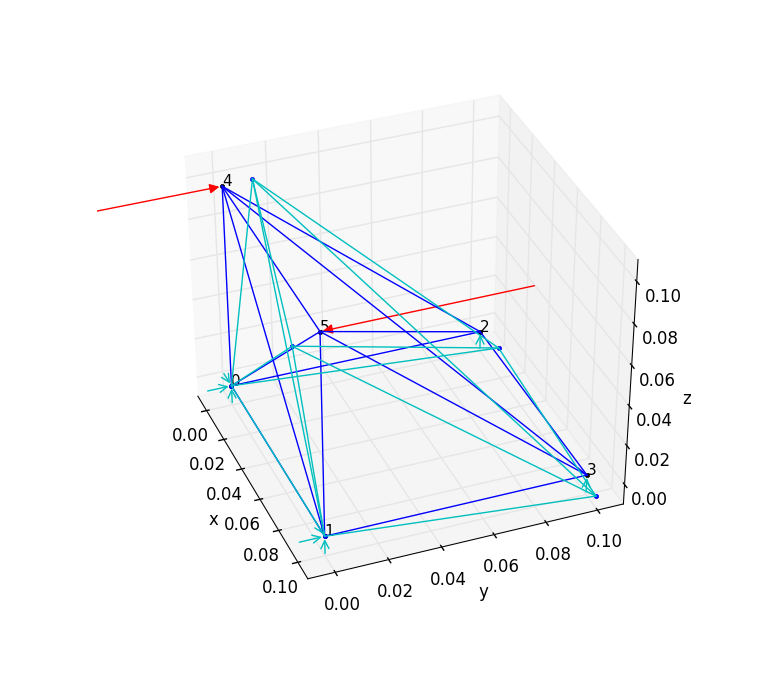
\includegraphics[width=\textwidth]{Verification/FEALink/3dVerification2.png}
    \caption{FEALink Model and Deformation}
    \label{fig:3dV2FEALink1}
  \end{subfigure}
  %
  \begin{subfigure}[b]{.45\textwidth}
    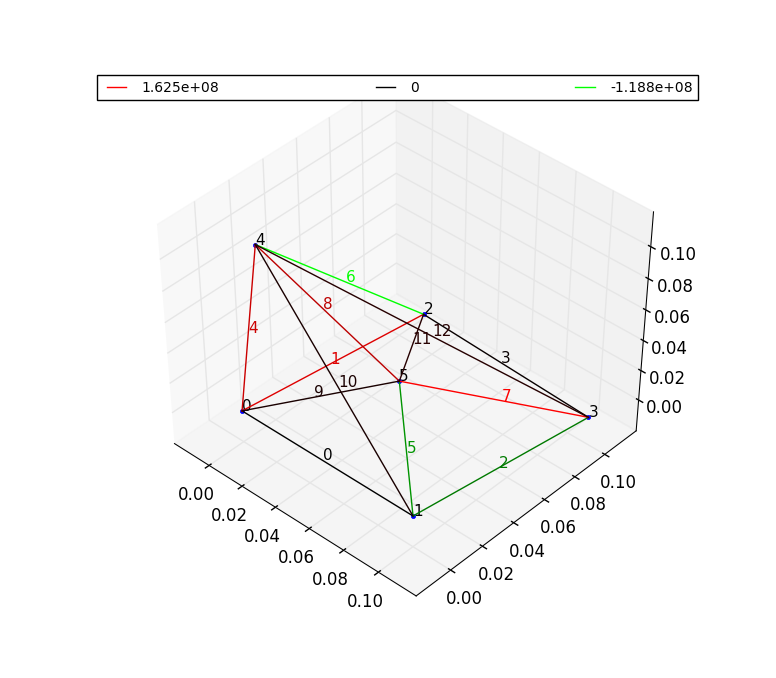
\includegraphics[width=\textwidth]{Verification/FEALink/3dVerification2_image2.png}
    \caption{FEALink Stress Results}
    \label{fig:3dV2FEALink2}
  \end{subfigure}
  %
  \begin{subfigure}[b]{0.45\textwidth}
    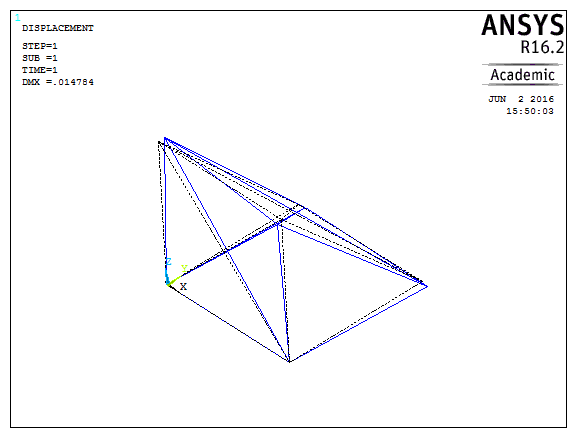
\includegraphics[width=\textwidth]{Verification/Ansys/3dVerification2.png}
    \caption{Ansys}
    \label{fig:3dV2Ansys}
  \end{subfigure}
\caption{3d Verification 2}
\label{fig:3dVerification2}%
\end{figure}

\begin{table}[h]
\centering
\caption{3d Verification 2 Displacement}
\label{table:3dV2}
\begin{tabular}{l|l|l|l|l|l|l}
Node & FEALink x & FEALink y & FEALink z & Ansys x  & Ansys y   & Ansys z   \\ \hline
0-1  & 0 m       & 0 m       & 0 m       & 0 m      & 0 m       & 0 m       \\
2    & .01457 m  & .00250 m  & 0 m       & .01457 m & .00250 m  & 0 m       \\
3    & .01457 m  & -.00250 m & 0 m       & .01457 m & .00250 m  & 0 m       \\
4    & .00250 m  & .01207 m  & .00250 m  & .00250 m & .01207 m  & .00250 m  \\
5    & .00250 m  & -.01207 m & -.00250 m & .00250 m & -.01207 m & -.00250 m
\end{tabular}
\end{table}

\end{document}  